\Chapter{Szimuláció}


\section{Adatbázisok és modellek}
A programban a drón, és telemetria adatmodell a legfontosabb.
Ezeket az adatokat olvassuk és mentjük,illetve szükségesek az azonosításhoz vagy bármilyen értelmes következtetéshez a problémához kapcsolódóan.

\subsection{Modellek az adatközpont programban}
\subsubsection{Telemetria modell}
A programban a telemetria modell a következőképpen néz ki:

\begin{python}
    package models

    import "time"

    type Telemetry struct {
        Speed              float64          `json:"speed" db:"speed"`
        Location           GPS              `json:"location"`
        Altitude           float64          `json:"altitude"`
        Bearing            float64          `json:"bearing"
        Acceleration       float64          `json:"acceleration"`
        BatteryLevel       int              `json:"battery_level"`
        BatteryTemperature int              `json:"battery_temperature"`
        MotorTemperatures  []int            `json:"motor_temperatures"`
        Errors             []TelemetryError `json:"errors" db:"errors"`
        TimeStamp          time.Time        `json:"time_stamp"`
        DroneID            int              `json:"drone_id"`
    }

    type TelemetryError int

    const (
        MotorFailure TelemetryError = iota
        BeaconSignalStrengthLow
        BeaconSignalInterference
        BeaconTemperatureTooHigh
        GPSInt	eference
        GPSSignalLost
        GPSTemperatureTooHigh
        ProcessorTemperatureTooHigh
        BatteryFailure
        FailedToEjectPackage
        PackageLost
        DestinationDistanceTooFar
    )

    type GPS struct {
        Latitude  float64 `json:"latitude" bson:"latitude"`
        Longitude float64 `json:"longitude" bson:"longitude"`
    }

\end{python}


\subsubsection{Drón modell}
A DDD-ben leírt elvek alapján, a drón modell mindenféleképp egy Entity-nek felel meg.
\begin{python}
    type Drone struct {
        ID           int           `json:"id" db:"drone_id" bson:"id"`
        Telemetry    Telemetry     `json:"telemetry" bson:"telemetry"`
        Parcel       Parcel        `json:"parcel"`
        Destinations []Destination `json:"destinations"`
        Consumption  float64       `json:"consumption"`
        Weight       float64       `json:"weight"`
        State        DroneState    `db:"state" bson:"state"`
    }

    type DroneState string

    const (
    DroneFree     DroneState = "free"
    DroneInFlight DroneState = "in-flight"
    )
\end{python}


\subsubsection{Parcel modell (szállítandó csomag)}
A drónok által szállított csomag így néz ki:
\begin{python}
    type Parcel struct {
        ID            int             `json:"id" db:"id" bson:"id"`
        TrackingID    string          `json:"tracking_id" `
        Name          string          `json:"name" db:"name" bson:"name"`
        Weight        float64         `json:"weight" db:"weight"`
        Location      GPS             `json:"location" bson:"location"`
        FromAddress   ShippingAddress `json:"from_address"`
        ToAddress     ShippingAddress `json:"to_address"`
        DropOffSite   GPS             `bson:"drop_off_site" `
        AssignedDrone int             `json:"assigned_drone" `
    }
\end{python}

\subsection{Relációs adatbázis, PostgreSQL}
A relációs adatbázissal is működik a szimuláció.
\paragraph{Relációs modell \ref{fig:postgres} } \mbox{} \\

\begin{figure}[h]
    \centering
    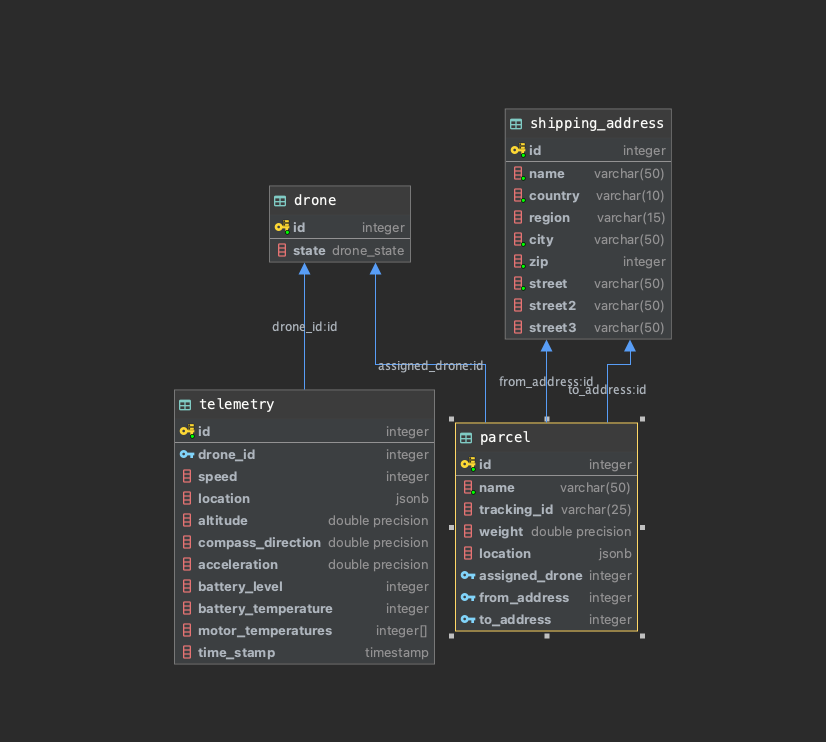
\includegraphics[scale=0.4]{images/postgres.png}
    \caption{PostgreSQL adatbázis modell}
    \label{fig:postgres}
\end{figure}

%TODO: Esetleg Er model


\subsubsection{Lost Update probléma}
A legtöbb relációs adatbázis támogatja a tranzakciókat. A tranzakciók ACID tulajdonságokkal bírnak.
Adatbázisok esetén az ACID az Atomicity (atomiság), Consistency (konzisztencia), Isolation (izoláció), és Durability (tartósság) rövidítése. Ezek nélkül az adatbázis integritása nem garantálható.
A PostgreSQL többféle izolációs szintet biztosít a tranzakciókhoz \cite{postgresql}. A Lost Update problémát garantáltan megoldja a PostgreSQL `Serializable` izolációs szintje.
\begin{table}[h]
    \centering
    \caption{ Standard SQL Transaction Isolation Levels}
    \begin{tabular}{l|c|c|c|}
Isolation Level & Dirty Read  & Nonrepeatable Read & Phantom Read\\
        \hline
Read uncommitted  & Possible & Possible & Possible \\
\hline
Read committed & Not possible & Possible & Possible \\
\hline
Repeatable read & Not possible & Not possible & Possible \\
\hline
Serializable & Not possible & Not possible & Not Possible \\
        \hline
    \end{tabular}
\end{table}

\subsubsection{PostgreSQL telepítése az alkalmazáshoz}\label{subsubsec:postgresql-telepítése-a-programhoz}

Ha nem található a fejlesztői környezetünkben PostgreSQL adatbázis, akkor \href{https://www.postgresql.org/download/}{telepíteni kell azt}.
Az adatbáziskezelőhöz csatlakozva, le kell futtatni a következő SQL scriptet.

\begin{lstlisting}[language=sql]
    CREATE TYPE drone_state AS ENUM ('free', 'in-flight');
    CREATE TABLE drone
    (
    id          SERIAL PRIMARY KEY,
    state       drone_state      DEFAULT 'free',
    weight      DOUBLE PRECISION default 4,
    consumption DOUBLE PRECISION DEFAULT 500
    );

    CREATE TABLE warehouse
    (
    id  SERIAL PRIMARY KEY,
    location_latitude DOUBLE PRECISION DEFAULT 48.080922,
    location_longitude DOUBLE PRECISION DEFAULT 20.766208
    );

    CREATE TABLE shipping_address
    (
    id      SERIAL PRIMARY KEY,
    name    VARCHAR(50) NOT NULL,
    country VARCHAR(10) NOT NULL,
    region  VARCHAR(15) DEFAULT NULL,
    city    VARCHAR(50) NOT NULL,
    zip     INT         NOT NULL,
    street  VARCHAR(50) NOT NULL,
    street2 VARCHAR(50) DEFAULT NULL,
    street3 VARCHAR(50) DEFAULT NULL
    );

    CREATE TABLE parcel
    (
    id                 SERIAL PRIMARY KEY,
    name               VARCHAR(50) NOT NULL,
    tracking_id        VARCHAR(25)               default '',
    weight             DOUBLE PRECISION          default 1,
    drop_off_latitude  DOUBLE PRECISION          DEFAULT 0,
    drop_off_longitude DOUBLE PRECISION          DEFAULT 0,
    assigned_drone     INT REFERENCES drone (id) DEFAULT NULL,
    from_address       INT REFERENCES shipping_address (id),
    to_address         INT REFERENCES shipping_address (id)
    );

    CREATE TABLE telemetry
    (
    id                  SERIAL PRIMARY KEY,
    drone_id            INT REFERENCES drone (id),
    speed               DOUBLE PRECISION DEFAULT 0,
    latitude            DOUBLE PRECISION DEFAULT 0,
    longitude           DOUBLE PRECISION DEFAULT 0,
    altitude            DOUBLE PRECISION default 1,
    bearing             DOUBLE PRECISION DEFAULT 0,
    acceleration        DOUBLE PRECISION DEFAULT 0,
    battery_level       INT              DEFAULT NULL,
    battery_temperature INT              DEFAULT NULL,
    motor_temperatures  INTEGER[],
    errors              INTEGER[],
    time_stamp          timestamp        DEFAULT NULL
    );
    INSERT INTO warehouse (id) VALUES (1);
\end{lstlisting}


\subsection{Dokumentum alapú adatbázis, MongoDB}

\subsubsection{Vizualizáció}

\begin{figure}[hbt!]
    \centering
    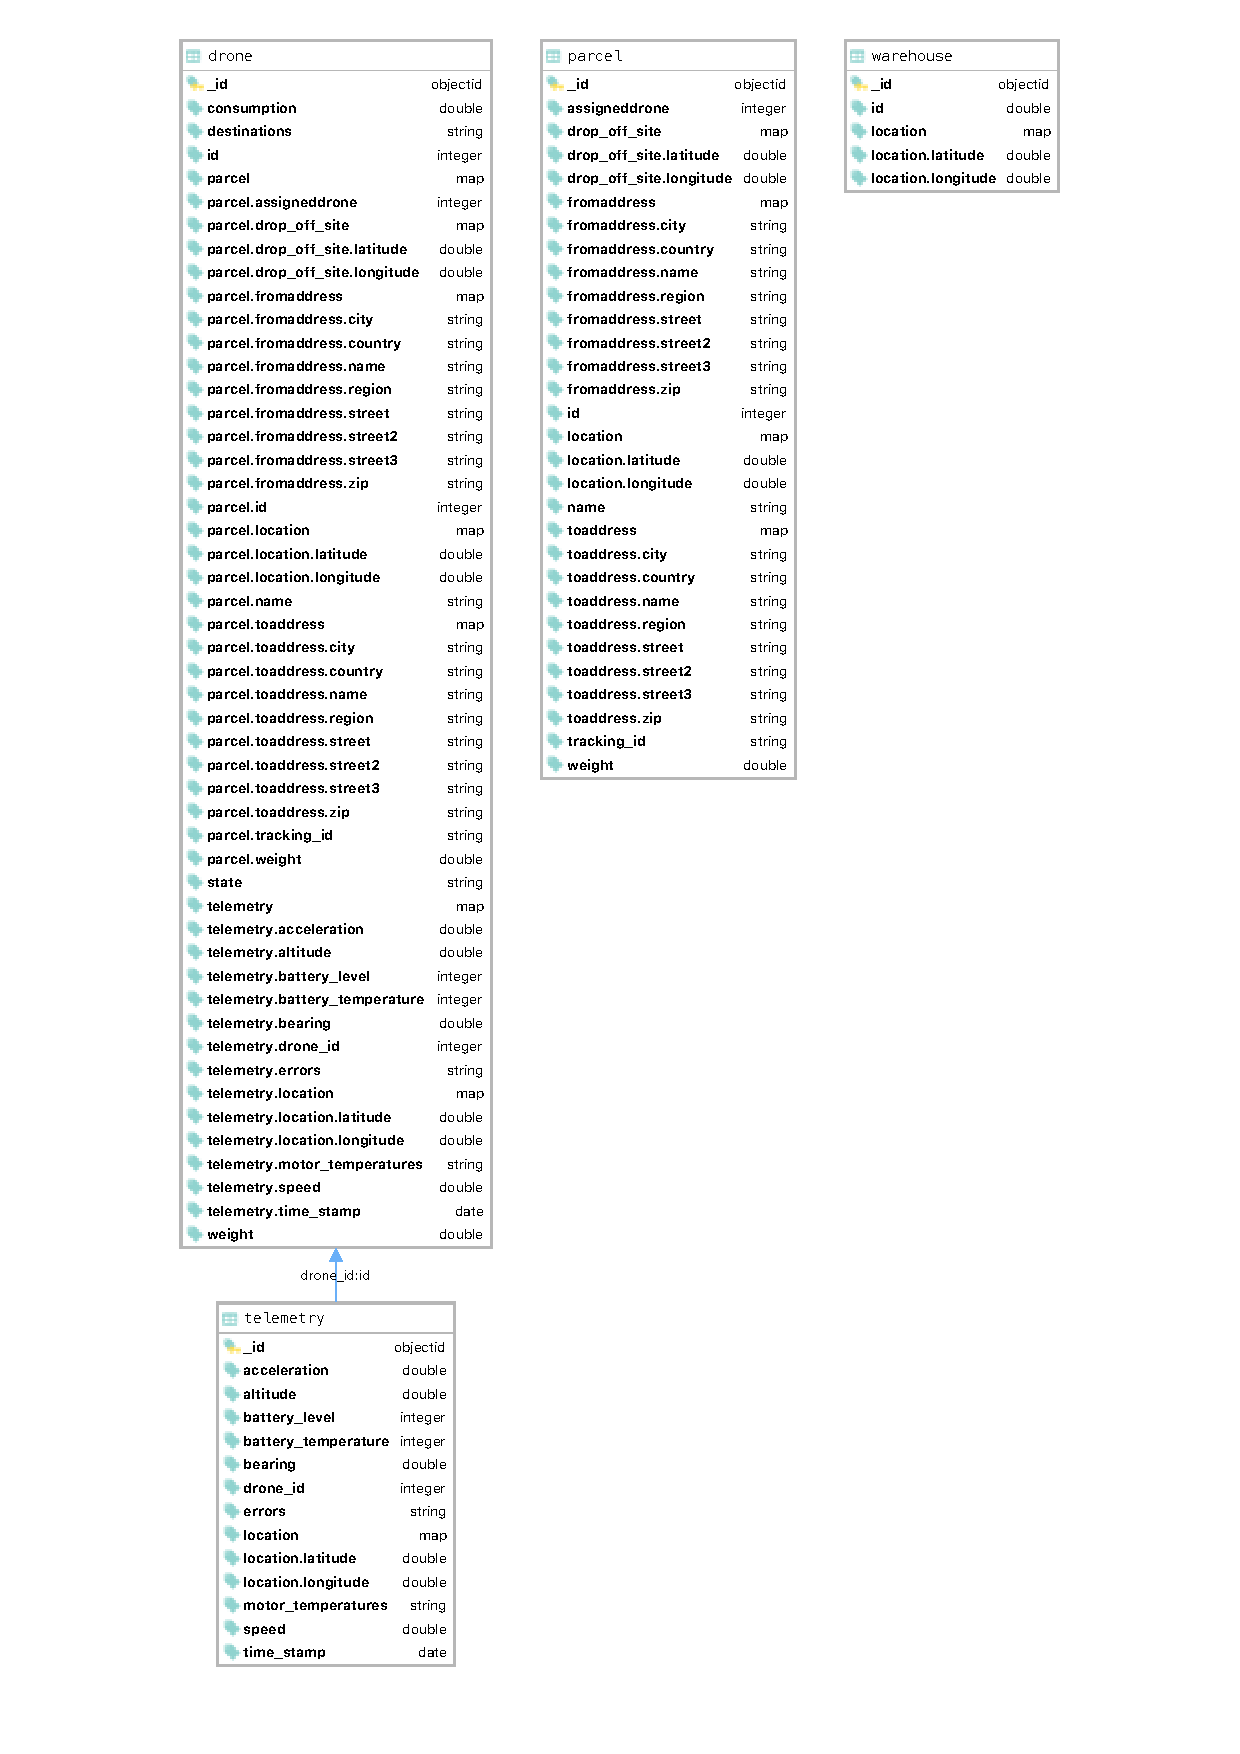
\includegraphics[scale=0.7]{images/mongo.pdf}
    \caption{MongoDB adatbázis vizualizáció}
    \label{fig:mongodb}
\end{figure}

\subsubsection{MongoDB telepítése az alkalmazáshoz}\label{subsubsec:mongodb-telepítése-az-alkalmazáshoz}
Ha nem található a fejlesztői környezetünkben MongoDB adatbázis, akkor \href{https://www.mongodb.com/try/download/community}{telepíteni kell azt}.
Az adatbáziskezelő konzolján keresztül le kell futtatni a következő két parancsot, egy megfelelő jogosultságú felhasználóval.
Ez egyik parancs létrehozza a drone\_delivery adatbázist, a másik parancs létrehoz nekünk egy felhasználót az előbb létrehozott adatbázishoz.
A későbbiekben ezzel a felhasználóval csatlakozunk az adatbázishoz.

\begin{python}
    use drone_delivery
\end{python}

\begin{python}

    db.createUser(
        {
        user: "drone-user",
        pwd: "drone-pwd",
        roles: [
            {
            role: "readWrite",
            db: "drone_delivery"
        }
        ]
    }
    )
\end{python}

\Section{Szimuláció működésének folyamata}

A szimuláció működése azzal kezdődik, hogy elindítjuk az adatközpont programot.
Felcsatlakozik az adatbázisokra, majd létrehozza a szervizeket, és a REST API-n várja a bejövő kéréseket.
Ez lehet például egy konfigurációs kérés, a drónok lekérdezése, vagy a szállítás indítása.

Közben a drón-raj program is elindul, ez a program is egy REST API-n várja a kéréseket.
A drón raj program az API-n megkapja a drónokat és a hozzájuk rendelt csomagokat, majd megkezdódik a szimuláció, a drón-raj program telemetria adatokat küld az adatközpont programnak.
A drón-raj program olyan telemetria adatokat fog generálni, amelyek minél jobban a valsóságot tükrözik és ezeket az adatokat tovább fogja küldeni az adatközpontnak.
\begin{python}
{
    "telemetry": {
    "speed": 2,
    "location": {
        "latitude": 48.08092020178216,
        "longitude": 20.766208061642047
    },
    "altitude": 50,
    "bearing": 178.68412647009515,
    "acceleration": 0,
    "battery_level": 98,
    "motor_temperatures": [
    41,
    43
    ],
    "time_stamp": "2021-04-01T15:04:05.630Z",
    "drone_id": 2
}
}
\end{python}

Ezeket a telemetria adatokat az adatközpont program fogadja a megadott porton és lementi az adott adatbázisba. \ref{fig:adatkozpont-flow}

\begin{figure}[h]
    \centering
    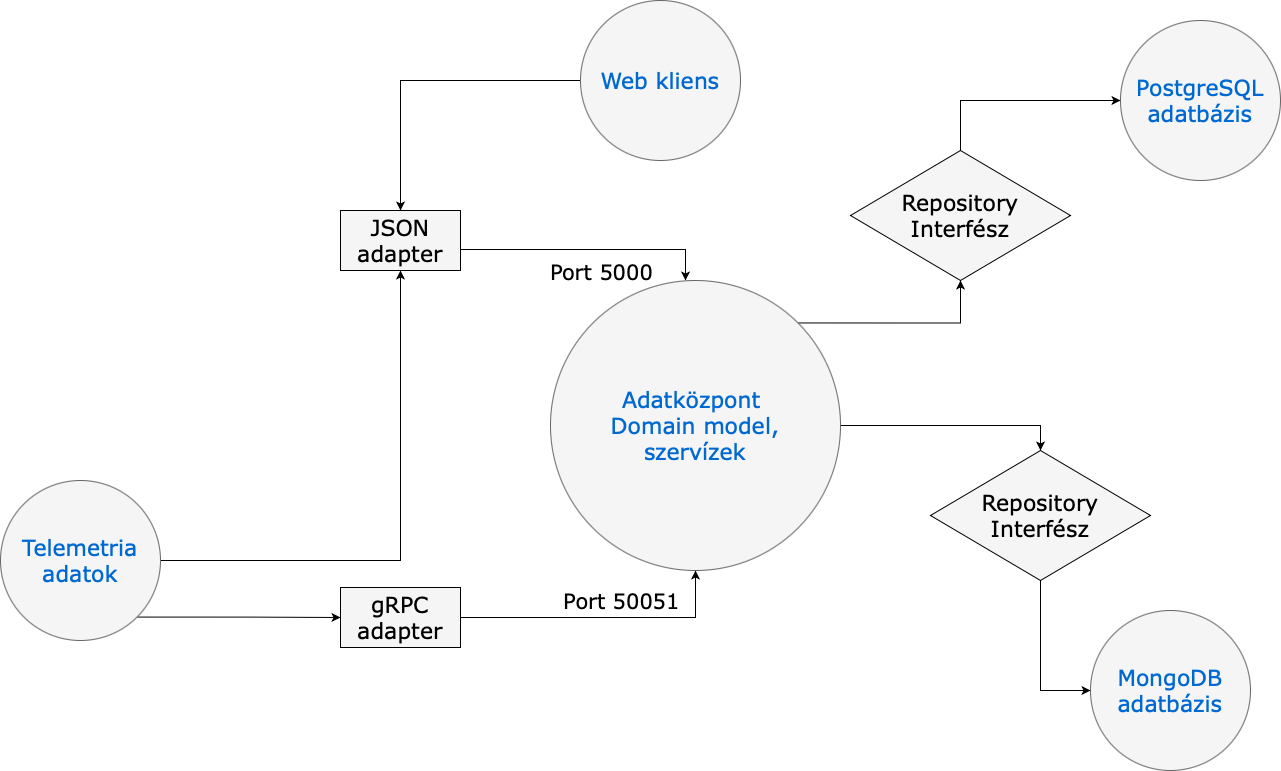
\includegraphics[scale=0.3]{images/adatkozpont-flow.png}
    \caption{Adatközpont program működésének folyamata}
    \label{fig:adatkozpont-flow}
\end{figure}

\section{A rendszer felépítése a követelmények alapján}
%TODO: ide irni Hexagonal arch. es DDD implementaciojarol. Beszurni kodot ahol latszik a repository, interface
\subsubsection{Szerkezeti felépítés}
Az alkalmazás jegyzék struktúráját a következő ábra \ref{fig:szerkezet} mutatja.
A drone-delivery jegyzék a program gyökér jegyzéke, itt található a docker-compose.yml fájl, ami az indításhoz szükséges.
A backend/server tartalmazza az adatközpont programot és a backend/drone-swarm a drón-raj programot.
Mindkét jegyzéknek hasonló a felépítése.
A cmd jegyzékbe van az indító main függvény.
A pkg jegyzék tartalmazza a kódbázis nagy részét, a domain és infrastuktúrához kapcsolódó részek itt helyezkednek el.
A pkg/domain/ben a domain kódbázis található, az infrastruktúrát és a hozzá tartozó adaptereket megvalósító kód a storage, network jegyzékekben van.
A drone-delivery/web-clientben található a web kliens, egy egyszerű html oldal ahonnan beállítjuk a szimulációt.

\begin{figure}[h]
    \centering
    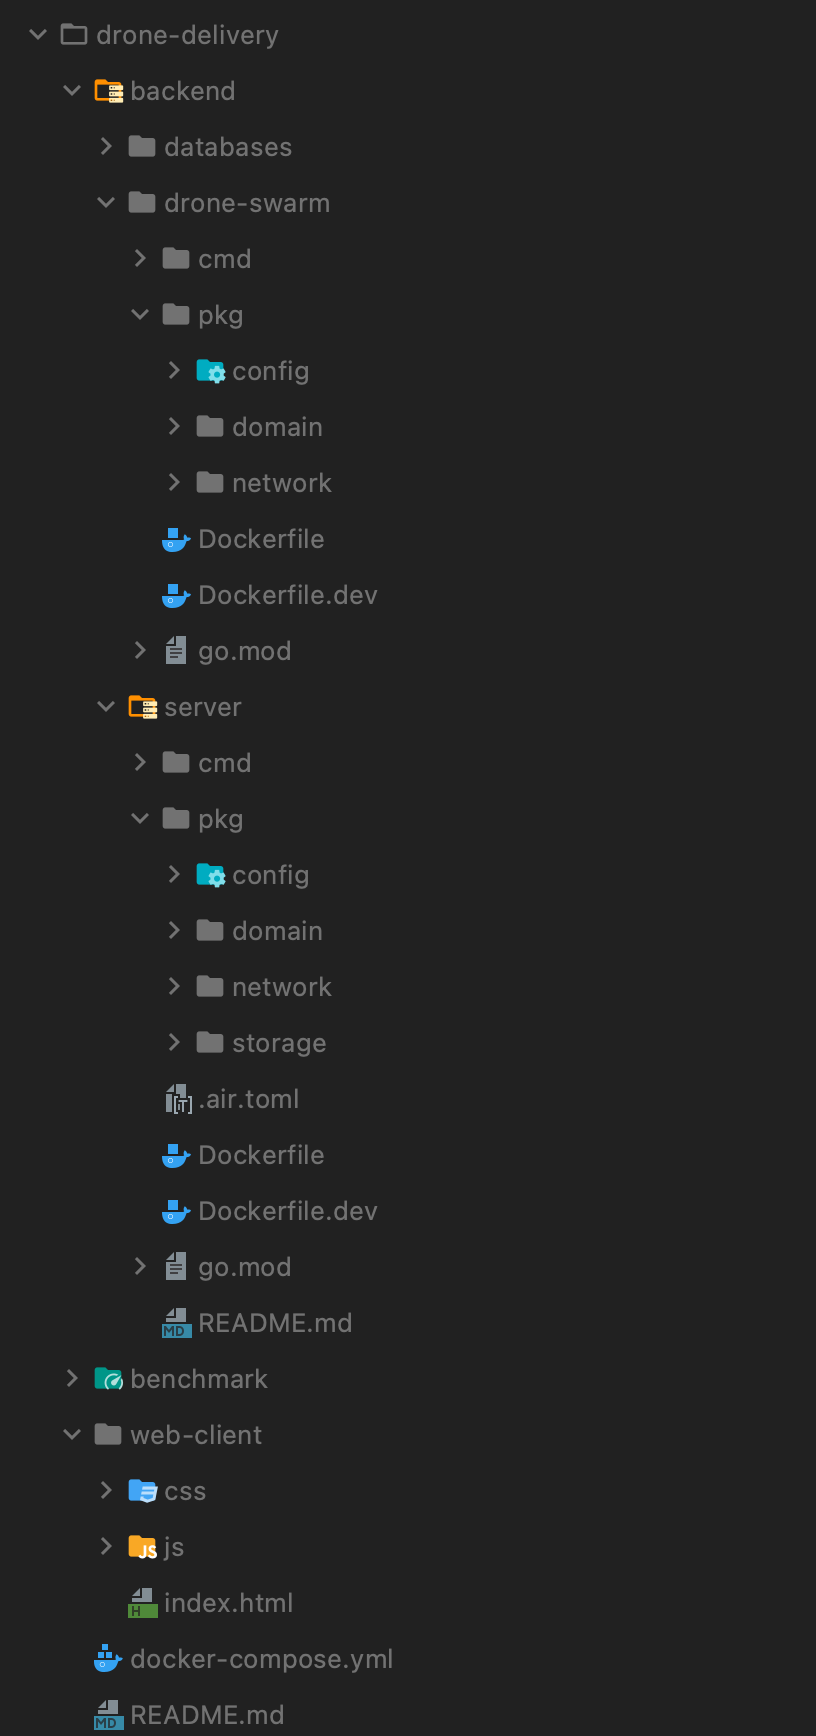
\includegraphics[scale=0.5]{images/szerkezet}
    \caption{Jegyzék szerkezet}
    \label{fig:szerkezet}
\end{figure}

\subsubsection{Portok és Adapterek, Domain Driven Design}
A hexagonal tervezési architektúra mindkét programban úgy került implementálásra, hogy a program magja, a domain üzleti logika a pkg/domain jegyzékben helyezkedik el.
Ez a domain jegyzék modellezi le az üzleti logika működését.
Itt találhatóak az interfészek, amik a hexagonal architektúra portjaiként szolgálnak, ezt kell implementálniuk az adaptereknek, így van összekötve a domain a különböző adapterekkel.
A DDD elemeit is megfigyelhetjük az elnevezésekből, valamint vannak Entity-k és Value Objectek.
\begin{python}
    # Entity
    type Drone struct {
        ID           int           `json:"id" db:"drone_id" bson:"id"`
        Telemetry    Telemetry     `json:"telemetry" bson:"telemetry"`
        Parcel       Parcel        `json:"parcel"`
        Destinations []Destination `json:"destinations"`
        Consumption  float64       `json:"consumption" db:"consumption" bson:"consumption"`
        Weight       float64       `json:"weight" db:"weight" bson:"weight"`
        State        DroneState    `db:"state" bson:"state"`
    }

    # Value Object
    type Destination struct {
        Coordinates          GPS
        ParcelDestination    bool
        WarehouseDestination bool
    }

    # Value Object
    type GPS struct {
        Latitude  float64 `json:"latitude" bson:"latitude"`
        Longitude float64 `json:"longitude" bson:"longitude"`
    }
\end{python}

\paragraph{Portok}\mbox{} \\
Minden szervízhez tartozik interface (port) amin az adapterek vagy más szervízek meghívhatják a szervíz metódusait.
Például az adatközpont drón szervízében olyan metódusok találhatóak amiket a REST API hív meg.
Itt a REST API az adapter, pontosabban vezérlő adapter.

\begin{python}
    type Service interface {
        DeliverParcels() error
        ProvisionDrone(wh models.Warehouse, d models.Drone) error
        GetFreeDrones() ([]models.Drone, error)
        GetDronesDelivering() ([]models.Drone, error)
        ChangeService(r Repository)
        ReinitializeDatabase(repos ...Repository) error
    }
\end{python}
Vezérelt adaptere az adatbázist és kimenő kommunikációt megvalósító adapterek.
Az adatközpont programban az adatbázisoknak a Repository interfészt kell implementálni, de a gRPC és JSON kommunikációhoz is tartozik interfész.
\begin{python}
    type Repository interface {
        GetFreeDrones() ([]models.Drone, error)
        GetParcelsInWarehouse() ([]models.Parcel, error)
        GetWarehouse() (models.Warehouse, error)
        GetDronesDelivering() ([]models.Drone, error)
        SetDroneState(droneID int, state string) error
        ReInitializeDeliveryData(drones []models.Drone, parcels []models.Parcel) error
    }

    type OutboundAdapter interface {
        FetchProvisionDroneEndpoint(wh models.Warehouse, d models.Drone) (success bool, err error)
    }
\end{python}

Ugyanígy a drón-raj programban.
\begin{python}
    type OutboundAdapter interface {
        SendTelemetryDataToServer(t models.Telemetry) error
    }
\end{python}
\paragraph{Adapterek} \mbox{} \\
Az adaptereket a portokon keresztül érjük el.
Alább a drón-raj program OutboundAdapter interfészét megvalósító adapter implementációját látjuk, gRPC-vel.
Csak azokat a részeket tartalmazza a példa ami szükséges a megértéshez.
Mivel a "SendTelemetryDataToServer(t models.Telemetry) error " metódus megtálható az adapterben, az interfész teljesül és az adapter használható a porton keresztül.
\begin{python}
    package grpc
    ...
    type Adapter struct {
        cc  *grpc.ClientConn
        tsc protobuf.TelemetryServiceClient
        streams map[int]StreamClient
    }

    func NewOutBoundAdapter() *Adapter {
        ...
    }

    func (a *Adapter) SendTelemetryDataToServer(t models.Telemetry) error {
        var err error
        var streamer protobuf.TelemetryService_TelemetryStreamClient
        ...
        telemetryDataRequest := protobuf.TelemetryDataRequest{
            Telemetry: &protobuf.Telemetry{
                Speed: t.Speed,
                Location: &protobuf.GPS{
                    Latitude:  t.Location.Latitude,
                    Longitude: t.Location.Longitude,
                },
                Altitude:           t.Altitude,
                Bearing:            t.Bearing,
                Acceleration:       t.Acceleration,
                BatteryLevel:       int32(t.BatteryLevel),
                BatteryTemperature: int32(t.BatteryTemperature),
                MotorTemperatures:  temperatures,
                Errors:             telemetryErrors,
                TimeStamp:          timestamppb.New(t.TimeStamp),
                DroneId:            int32(t.DroneID),
            },
        }
        err = streamer.Send(&telemetryDataRequest)
    }

\end{python}

Az adatközpont program MongoDB és PostgreSQL adatbázisához kapcsolódó, a Repository interfészt megvalósító adapterek a pkg/storage jegyzékben helyezkednek el.


\subsubsection{Dependency Injection}
A Hexagonal architektúra elvárja a kicserélhetőséget, laza kapcsolatokat és hogy az alkalmazás komponensek portokon kapcsolódjanak össze.
Ennek más előnyei is vannak, így lényegesen könnyebb a tesztelhetőség és karbantartás.
Arról már volt szó, hogy mik az adapterek és hogyan használjuk őket a portokon keresztül.
De arról még nem volt szó, hogy pontosan hogyan adjuk át az adaptereket, hogyan hivatkozunk az adapterekre.
Ehhez dependency injekciót használunk.
Azaz létrehozunk egy adaptert, szolgáltatást (szervíz) és azt átadjuk egy másik szolgáltatásnak, adapternek.
Olyan is előfordulhat, hogy a az alkalmazás domain részében két szolgáltatás egymás között portokon kommunikál.
Például a drón szolgáltatás létrehozásához szükséges paramétereket az alábbi kódrészletben láthatjuk.
Ezekből a paraméterekből a Repository, OutboundAdapter típusúak portok más adapterekhez.
Később a szolgáltatásban ezekre a portokra hivatkozunk, ezeken keresztül érjük el az adapterek metódusait.

\begin{python}
    func NewService(r Repository, ea OutboundAdapter, l gokitlog.Logger, rs routing.Service) *service {
        return &service{r, ea, l, rs}
    }
\end{python}

Az alábbi példán láthatjuk, hogy a postgreSQL, mongoDB adatbázisokat implementáló, és a külső kommunikációért felelős JSON adaptert átadjuk különböző szolgáltatásoknak.
Ezek rendre postgresStorage, mongoStorage, jsonAdapter.
\begin{python}
    postgresStorage, err := postgres.NewStorage(config.PostgresConfig)
    ...
    mongoStorage, err := mongodb.NewStorage(config.MongoConfig)
    ...
    jsonAdapter := outbound.NewJSONAdapter()
    geo := ellipsoid.Init("WGS84", ellipsoid.Degrees, ellipsoid.Meter, ellipsoid.LongitudeIsSymmetric, ellipsoid.BearingIsSymmetric)
    ...
    ts = telemetry.NewService(postgresStorage, logger, geo)
    rs = routing.NewService(logger)
    ds = drone.NewService(postgresStorage, jsonAdapter, logger, rs)
\end{python}

Majd a szolgáltásokat átadjuk egy vezérlő adapternek, egy REST API-nak ami kéréseket fogad és ez alapján a szolgáltatások portjain a megfelelő metódust meghívja.
\begin{python}
    router := rest.Handler(ds, ts, postgresStorage, mongoStorage)
\end{python}

%TODO: szekvencia diagramok is a mukodesrol, a kodban. Main fgv. -> newservice ... -> rest es grpc endpoint

\subsubsection{Konfiguráció}
A konfiguráció beállításáért a config csomag felel.
Az adatközpont, és drón-raj programban is található egy SetConfig függvény a config csomagban.
Ez környezeti változókat olvas ki, és az alapján beállítja a megfelelő értékeket.
A környezeti változókat a docker-compose.yml fájlban tudjuk módosítani.

\begin{python}
    func SetConfig() {
        flag.StringVar(&DroneSwarmURL, "drone swarm domain url", os.Getenv("DRONE_SWARM_URL"),
        "An url for the drone swarm application, with protocol")

        PostgresConfig.UserName = os.Getenv("PGUSER")
        PostgresConfig.Database = os.Getenv("PGDATABASE")
        PostgresConfig.Host = os.Getenv("PGHOST")
        PostgresConfig.Port = os.Getenv("PGPORT")
        PostgresConfig.SSSLMode = os.Getenv("PGSSL")
        PostgresConfig.PW = os.Getenv("PGPASSWORD")

        MongoConfig.UserName = os.Getenv("MONGO_USER")
        MongoConfig.Database = os.Getenv("MONGO_DB")
        MongoConfig.Host = os.Getenv("MONGO_HOST")
        MongoConfig.Port = os.Getenv("MONGO_PORT")
        MongoConfig.PW = os.Getenv("MONGO_PWD")
    }
\end{python}

\begin{python}
    func SetConfig() {
        flag.StringVar(&ServerHTTPDomain, "server domain for http", os.Getenv("SERVER_DOMAIN"), "domain of server, with protocol")
        flag.StringVar(&ServerHTTPPort, "server port for http", os.Getenv("SERVER_PORT"), "the port the server is listening on")
        flag.StringVar(&ServerGRPCDomain, "server domain for grpc", os.Getenv("SERVER_GRPC_DOMAIN"), "domain of server, with protocol")
        flag.StringVar(&ServerGRPCPort, "server port for grpc", os.Getenv("SERVER_GRPC_PORT"), "the port the server is listening on")

        PostgresConfig.UserName = os.Getenv("PGUSER")
        PostgresConfig.Database = os.Getenv("PGDATABASE")
        PostgresConfig.Host = os.Getenv("PGHOST")
        PostgresConfig.Port = os.Getenv("PGPORT")
        PostgresConfig.SSSLMode = os.Getenv("PGSSL")
        PostgresConfig.PW = os.Getenv("PGPASSWORD")
    }
\end{python}



\section{Az rendszer működése}

A rendszer úgy működik, hogy először elindul az adatközpont program, felcsatlakozik az adatbázisokra, létrejönnek a vezérelt adapterek.
Ezeket az adaptereket átadjuk a szolgáltatásoknak. Létrehozzuk a vezérlő adaptereket, ezeknek az adaptereknek átadjuk a szolgáltatásokat.
A két vezérló adapter az adatközpontban a REST API ami 5000-es porton hallgat, illetve a gRPC végpont ami 50051-es porton hallgat.
A drón raj program elindul, hasonló módon mint az adatközpont programban, először a vezérelt adapterek, majd a vezérlő adapterek jönnek létre.
Létrejön a gRPC kapcsolat az adatközpont és drón-raj program között.
A drón raj program REST API-ja a 2000-es porton hallgat.
A web klienssel indíthatjuk a szimulációt, miután megnyitottuk a böngészővel, egy egyszerű kezelő felület fogad.

A folyamat \ref{fig:mukodes} röviden úgy néz ki, hogy:
\begin{enumerate}
    \item A web kliensben kiválasztjuk, hogy milyen protokollt és formátumot, valamint adatbázist szeretnénk használni. Alapértelmezettként PostgreSQL adatbázis és HTTP/1.1 protokoll JSON formátummal van kiválasztva.
    \item A szimuláció indítása gomb megnyomásával az adatközpont program REST API \textit{/api/delivery} végpontjára küld egy POST requestet a web kliens.
    \item Az adatközpont lekérdezi a drónokat és csomagokat, majd ezek alapján optimalizálja az útvonalakat.
        A drónoknak most már megvan a hozzájuk tartozó csomagjuk és az útvonal amin haladniuk kell.
    \item Ezt az információt az adatközpont elküldi egy POST requestben a drón raj program REST API \textit{/provision} végpontjára.
    \item A drón-raj program szimulálja a drónok működését, és telemetria adatokat küld az adatközpontnak JSON vagy gRPC formátumban, attól függ mit választottunk.
    \item Az adatközpont elmenti az adatokat PostgreSQL vagy MongoDB adatbázisba, attól függ melyikbe, hogy mit választottunk.
\end{enumerate}

\begin{figure}[h]
    \centering
    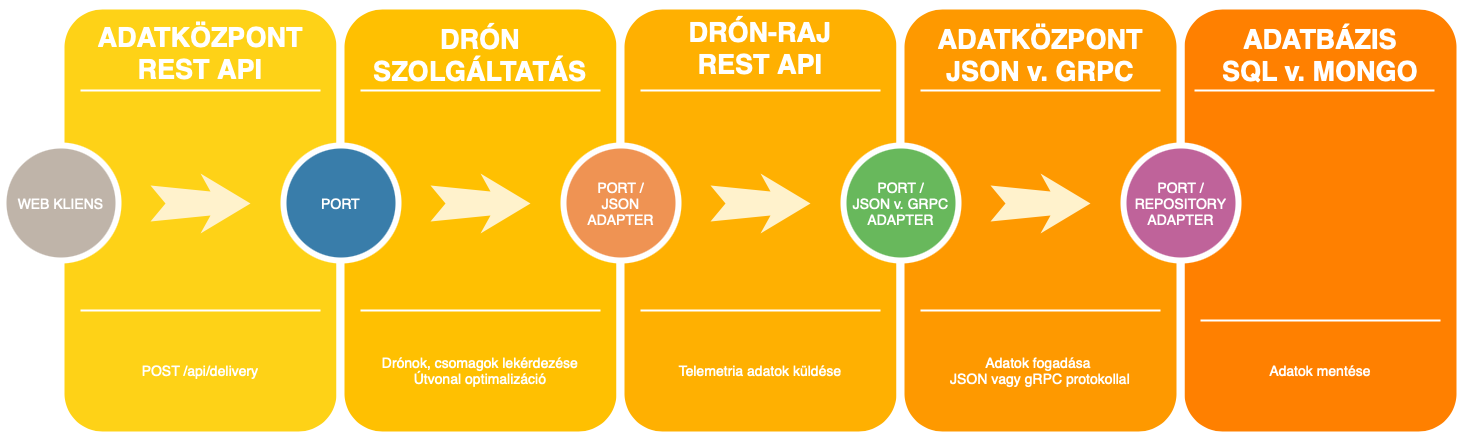
\includegraphics[scale=0.3]{images/mukodes}
    \caption{Az szimuláció folyamata}
    \label{fig:mukodes}
\end{figure}



\section{Telepítés, tesztelés}
\subsubsection{Adatbázisok elindítása}
A rendszer indítása úgy kezdődik, hogy megbizonyosodunk arról, hogy a MongoDB adatbázis és a PostgreSQL adatbázis fut és lehet rá csatlakozni.
Ha ez a 2 adatbáziskezelő nem található meg gépünkön, akkor először telepíteni kell őket.
Nálam a következőképp néz ki az indítás. A terminálban elindítom a MongoDB adatbázist.
\begin{lstlisting}[language=bash]
  $ brew services stop mongodb-community@4.4
\end{lstlisting}

Ezután a mongo parancsot kiadva kapcsolódom az adatbáziskezelő konzolos felületére.
Megbizonyosodom, hogy létezik a drone\_delivery adatbázis.
Ha nem létezik, lefuttatom a telepítéshez szükséges parancsokat \ref{subsubsec:mongodb-telepítése-az-alkalmazáshoz}.
\begin{lstlisting}[language=bash]
  $ mongo
\end{lstlisting}


Ezután elindítok egy PostgreSQL 11 vagy újabb verziójú PostgreSQL adatbázist, a fejlesztői környezetemben ez egy Postgres nevű grafikus kezelőfelületű program által történik.
Megbizonyosodok arról, hogy létezik a dbdrone\_delivery adatbázis, és létezenek a megfelelő táblák. Ha nem léteznek, lefuttatom telepítéshez szükséges scriptet \ref{subsubsec:postgresql-telepítése-a-programhoz}.

\subsubsection{Alkalmazás indítása Dockerrel}
Az alkalmazást Docker konténerben indítom el a teszteléshez, így minden fejleszői környezetében elindul, ahol van telepítve a Docker.
Az indításhoz elengedhetetlen 2 feltétel teljesülése: az adatbázisok futnak, és a \textit{docker-compose.yml} fájlban a megfelelő konfiguráció van beállítva.
A \textit{drone-delivery} jegyzékben, a terminálban kiadom a következő parancsot.
\begin{lstlisting}[language=bash]
  $ docker-compose up --build
\end{lstlisting}

Ez megépíti a konténereket, letölti a szoftver függőségeket illetve csomagokat, majd a konténerekben elindulnak a programok.
Ezután nincs más dolgunk, mint a \textit{drone-delivery/web-client} jegyzékben található \textit{index.html} fájlt megnyitni a böngészőben, az egyértelmű kezelőfelülettel tudjuk konfigurálni és indítani a szimulációt.

\section{Szállítási probléma a programban}
\subsubsection{Az adatközpont távolság számítása}
Az adatközpont program az Ortodroma számítást használja, hogy kiszámolja a távolságot a legoptimálisabb útvonal keresése közben.
\begin{python}
    func (s *service) CalculateDistance(lat1, lng1, lat2,
    lng2 float64, unit ...string) float64 {
        const PI = float64(math.Pi) //3.141592653589793

        radlat1 := PI * lat1 / 180
        radlat2 := PI * lat2 / 180

        theta := lng1 - lng2
        radtheta := PI * theta / 180

        dist := math.Sin(radlat1)*math.Sin(radlat2) +
        math.Cos(radlat1)*math.Cos(radlat2)*math.Cos(radtheta)

        if dist > 1 {
            dist = 1
        }

        dist = math.Acos(dist)
        dist = dist * 180 / PI
        dist = dist * 60 * 1.1515

        if len(unit) > 0 {
            if unit[0] == "K" {
                dist = dist * 1.609344
            } else if unit[0] == "N" {
                dist = dist * 0.8684
            } else if unit[0] == "METER" {
                dist = dist * 1.609344 * 1000
            }
        }

        return dist
    }
\end{python}
\subsubsection{A drón-raj program számításai}
A pontos szimulációs értékekhez egy könyvtárat használunk, ami megfelel a WGS84 GPS rendszernek.
Ezzel a könyvtárral pontos adatokat tudunk generálni a drón helyzetéről, irányáról.

\begin{python}
    geo := ellipsoid.Init("WGS84", ellipsoid.Degrees, ellipsoid.Meter,
    ellipsoid.LongitudeIsSymmetric, ellipsoid.BearingIsSymmetric)
    routingService := routing.NewService(geo)
\end{python}

Ezután a útvonalakért felelős szervízben két metódussal számoljuk ki a szükséges értékeket.
A \textit{CalculateDroneDistanceAndDirectionFromDestination} metódussal adott induló koordináták alapján megkapjuk a legrövidebb utat a célkoordinátákhoz, és az irányt is.
A \textit{CalculateDroneNextCoordinates} metódus megmondja adott induló koordináták és távolság valamint irány alapján hogy hova érkezünk, azaz a célkoordinátákat.

\begin{python}
    func (s *service) CalculateDroneDistanceAndDirectionFromDestination(
    currentLat, currentLon, destinationLat, destinationLon float64)
    (distance, bearing float64) {
        distance, bearing = s.geometry.To(currentLat,
        currentLon, destinationLat, destinationLon)
        return distance, bearing
    }

    func (s *service) CalculateDroneNextCoordinates(lat, lon,
    dist, bearing float64) (nextLat,nextLon float64) {
        nextLat, nextLon = s.geometry.At(lat, lon, dist, bearing)
        return nextLat, nextLon
    }
\end{python}

\Section{Mérések}

Az alkalmazással kapcsolatban méréseket is végeztem, JMeter\cite{apache}  és ghz\cite{ghz} programokat használtam.
Ezeket a méréseket fogom bemutatni és összehasonlítani.
Összehasonlításra kerülnek az alkalmazásban használt különböző protokollok, formátumok és adatbázisok.
Minden mérés a telemetria adatok küldését és mentését ábrázolja, ugyanolyan körülmények között.
Üres adatbázissal, összesen 10000 telemetria adatot küldünk, 100 szálon.
Minden egyes méréshez tartozik egy rövid összegzés, hisztogramok a teljesítményről.

\subsection{JMeter}
A Jmeteres méréshez készítettem egy \textit{telemetria.jmx}\ref{fig:jmeter-meres} konfigurációs fájlt.
A mérést úgy állítottam be, hogy 100 szálon küldünk összesen 10000 db telemetria adatot.
\begin{figure}[h]
    \centering
    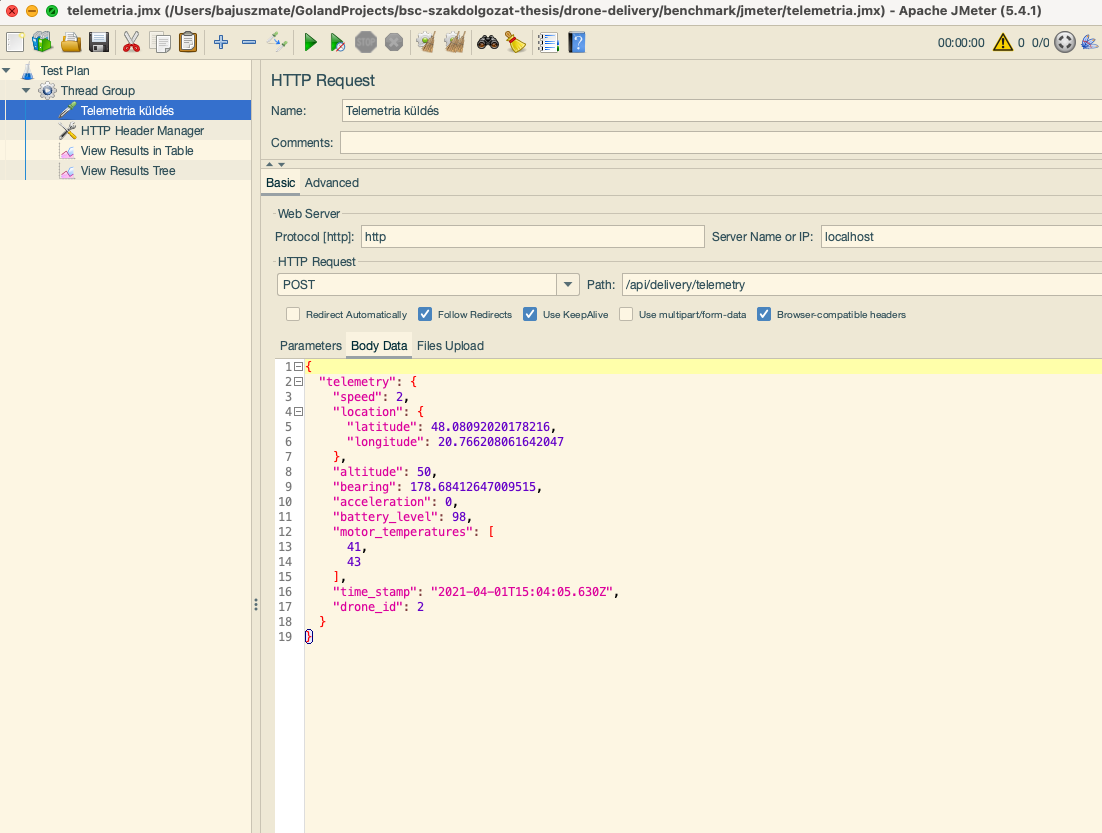
\includegraphics[scale=0.3]{images/jmeter-meres}
    \caption{Jmeter telemetria.jmx}
    \label{fig:jmeter-meres}
\end{figure}
Ez a \textit{drone-delivery/benchmark/jmeter} jegyzékben található.
A mérést úgy végeztem, hogy két jegyzékben lefuttattam a következő parancsot.
\begin{itemize}
    \item \textit{drone-delivery/benchmark/jmeter/mongo}
    \item \textit{drone-delivery/benchmark/jmeter/postgres}
\end{itemize}
\begin{lstlisting}[language=bash]
  $ jmeter -n -t ./../telemetria.jmx -l ./benchmark.csv -e -o  ./output
\end{lstlisting}

\subsubsection{HTTP/1.1 JSON, PostgreSQL adatbázissal}
\begin{figure}[hbt!]
    \centering
    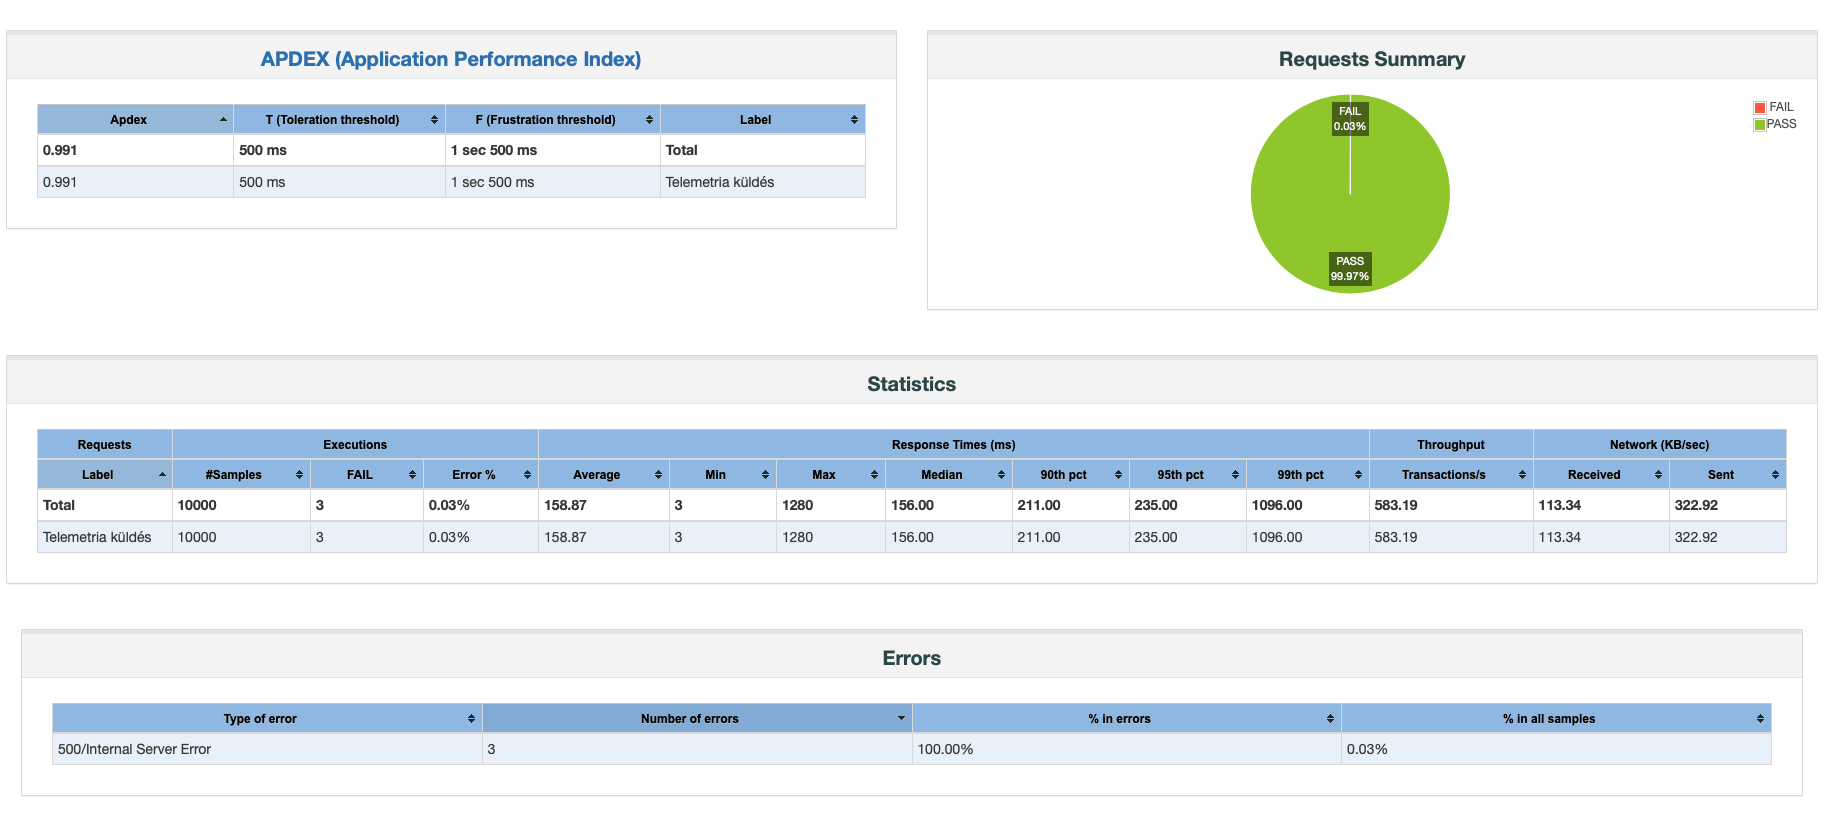
\includegraphics[scale=0.2]{images/jmeter-json-postgres}
    \caption{Jmeter mérései PostgreSQL adatbázissal HTTP/1.1 protokoll JSON formátummal}
    \label{fig:jmeter-json-postgres}
\end{figure}

\begin{figure}[hbt!]
    \centering
    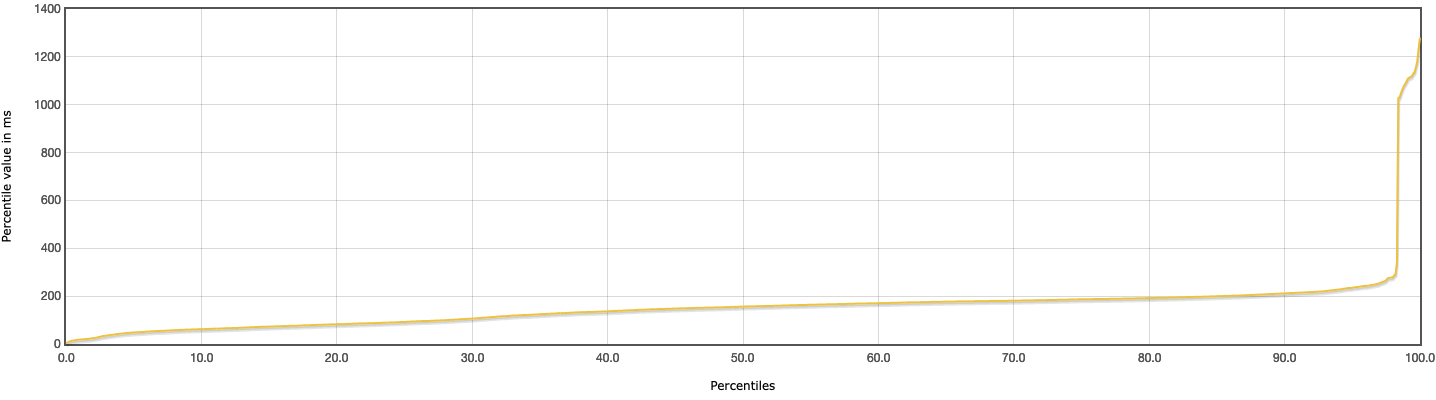
\includegraphics[scale=0.3]{images/json-postgres-response-times}
    \caption{Válaszidők PostgreSQL / JSON konfiguráció}
    \label{fig:json-postgres-response-times}
\end{figure}

\begin{figure}[hbt!]
    \centering
    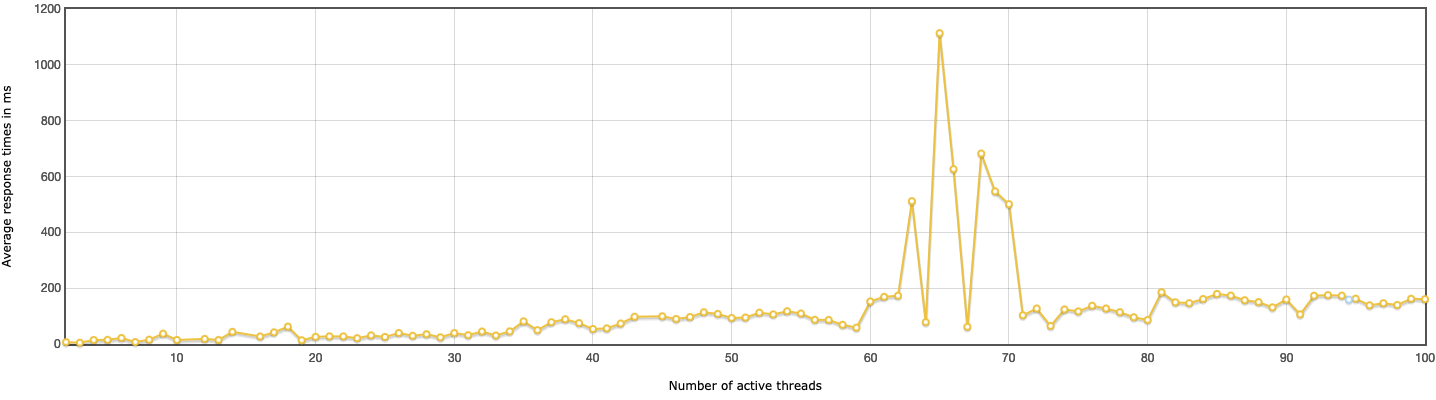
\includegraphics[scale=0.3]{images/json-time-vs-threads}
    \caption{Idő és szálak kapcsolata PostgreSQL / JSON konfiguráció}
    \label{fig:json-time-vs-threads}
\end{figure}

A mérés közben a PostgreSQL adatbázis nem tudta kezelni a túl sok kapcsolatot \ref{fig:jmeter-json-postgres}, így 3-szor hibával tért vissza a mentés.

\subsubsection{HTTP/1.1 JSON, MongoDB adatbázissal}
\begin{figure}[hbt!]
    \centering
    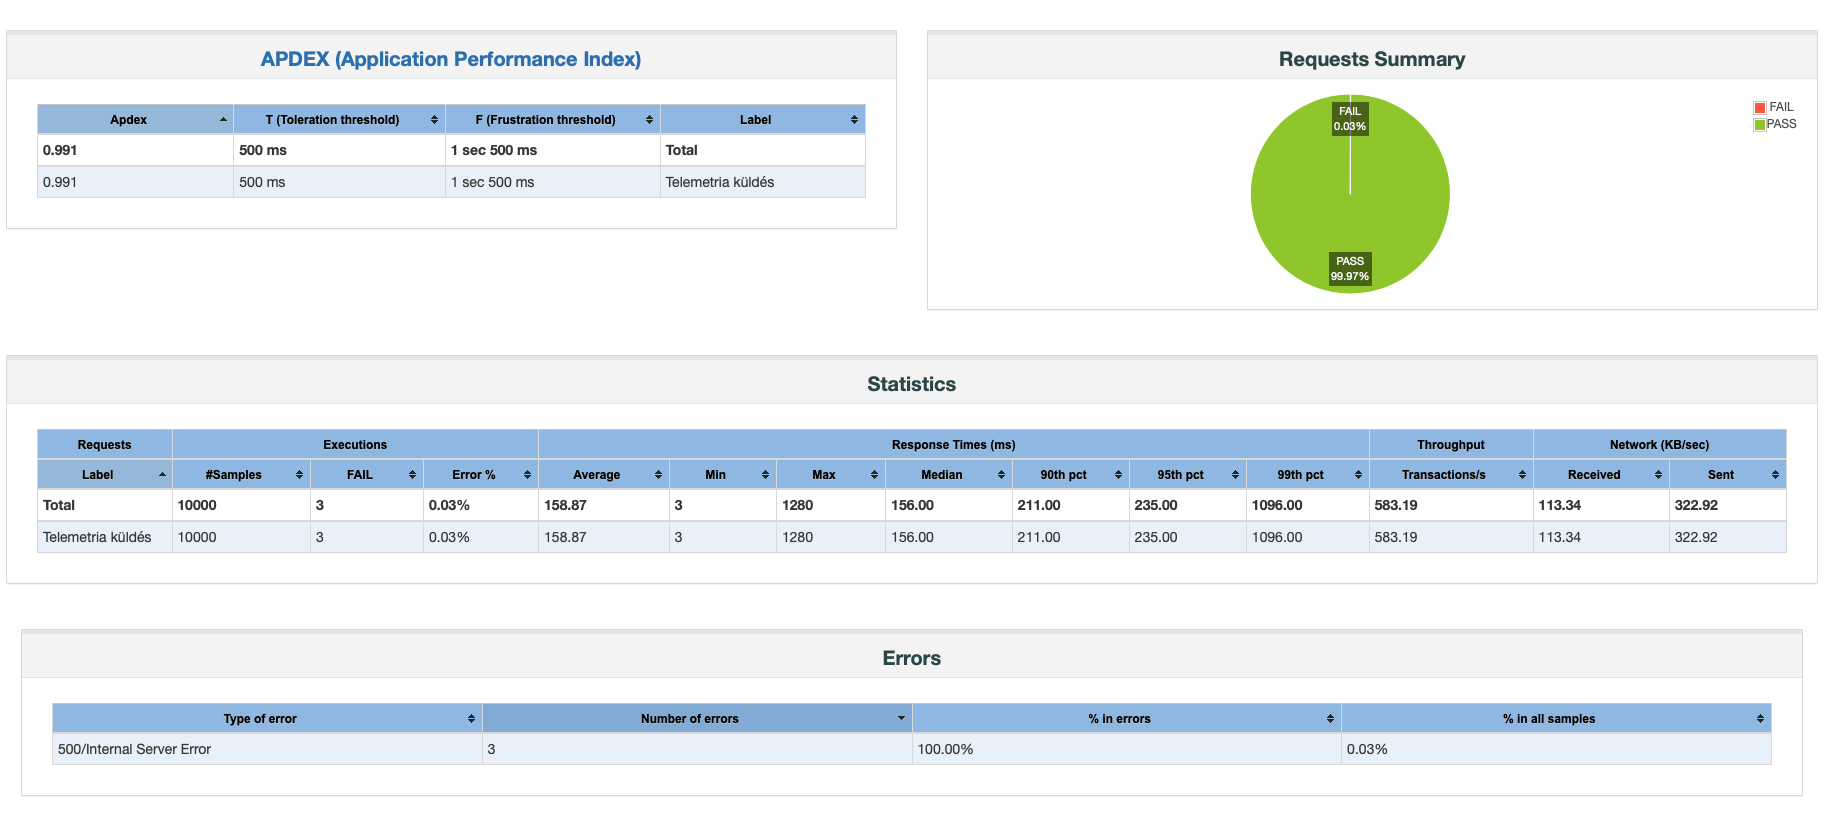
\includegraphics[scale=0.2]{images/jmeter-json-postgres}
    \caption{Jmeter mérései MongoDB adatbázissal HTTP/1.1 protokoll JSON formátummal}
    \label{fig:jmeter-json-mongo}
\end{figure}

\begin{figure}[hbt!]
    \centering
    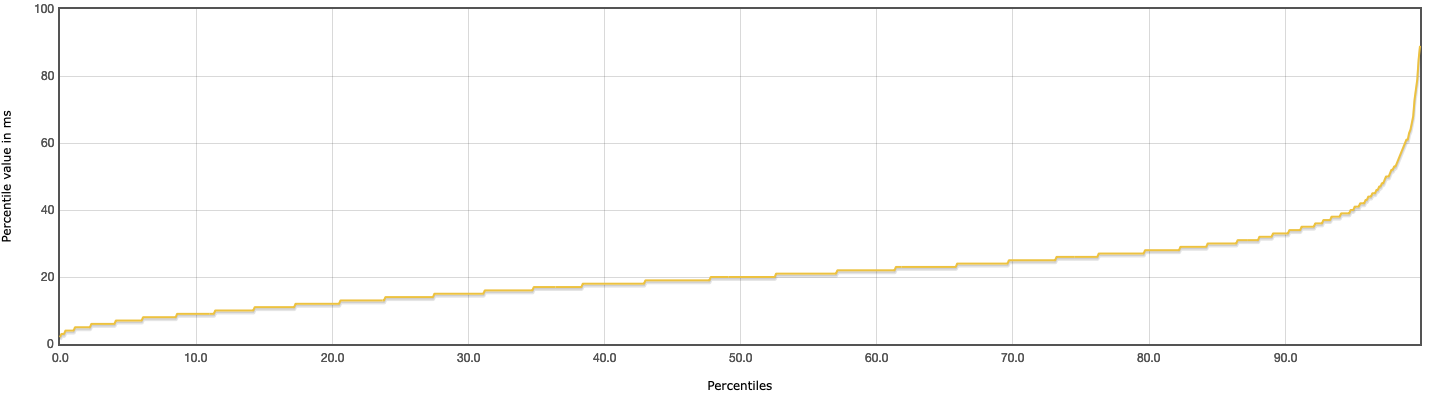
\includegraphics[scale=0.3]{images/json-mongo-response-times}
    \caption{Válaszidők MongoDB / JSON konfiguráció}
    \label{fig:json-mongo-response-times}
\end{figure}

\begin{figure}[hbt!]
    \centering
    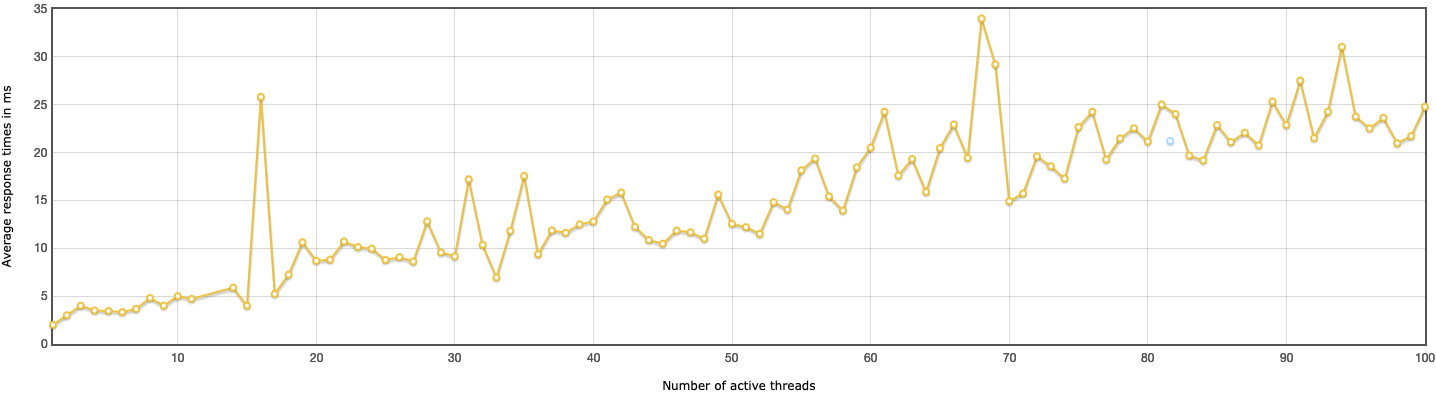
\includegraphics[scale=0.3]{images/json-mongo-time-vs-threads}
    \caption{Idő és szálak kapcsolata MongoDB / JSON konfiguráció}
    \label{fig:json-mongo-time-vs-threads}
\end{figure}
\begin{remark}
    A MongoDB adatbázis jobban teljesített mint a PostgreSQL.
    Az erőforrásokat is jobban használta ki, a mérések alapán azt a következtetést vonhatjuk le, hogy a PostgreSQL-ben sok konkurrens írás nem hatékony, a teljesítmény rovására megy.
\end{remark}

\subsection{ghz}
A ghz egy gRPC terhelés tesztelő program. Nincs hozzá grafikus felület.
Először \href{https://github.com/bojand/ghz}{feltelepítjük a ghz programot}, majd a következő paranccsal tudjuk tesztelni, a kliens oldali Telemetria streamelést az alkalmazásunkhoz.
Azaz itt a drón raj helyett a ghz program küldi a telemetria adatokat.
Az output formátumnak html-t adtam meg, a \textit{-c} paraméter a konkurrencia (szál) értéket jelöli, 100-at adtam meg.
A \textit{-n} paraméter requestek számát jelöli, ezt 10000-re állítottam.

\begin{lstlisting}[language=bash]
  $  ~ ghz -c 100 -n 10000 --format html --output report-gRPC-postgres.html  --insecure \
  --proto /Users/bajuszmate/go/src/github.com/bajusz15/ghz-benchmark/ghz/cmd/benchmark/protobuf/telemetry.proto \
  --call telemetry_grpc.TelemetryService.TelemetryStream \
  -d '[
  {
    "telemetry": {
      "speed": 2,
      "location": {
        "latitude": 48.08092020178216,
        "longitude": 20.766208061642047
      },
      "altitude": 50,
      "bearing": 178.68412647009515,
      "acceleration": 0,
      "battery_level": 98,
      "motor_temperatures": [],
      "time_stamp": "2021-04-01T15:04:05.630Z",
      "drone_id": 2
    }
  },
  {
    "telemetry": {
      "speed": 2,
      "location": {
        "latitude": 48.08092020178216,
        "longitude": 20.766208061642047
      },
      "altitude": 50,
      "bearing": 178.68412647009515,
      "acceleration": 0,
      "battery_level": 98,
      "motor_temperatures": [],
      "time_stamp": "2021-04-01T15:04:05.630Z",
      "drone_id": 2
    }
  }
]' \
  localhost:50051
\end{lstlisting}

\subsubsection{HTTP/2 gRPC, PostgreSQL adatbázissal \ref{fig:ghz-postgres}}

\begin{figure}[hbt!]
    \centering
    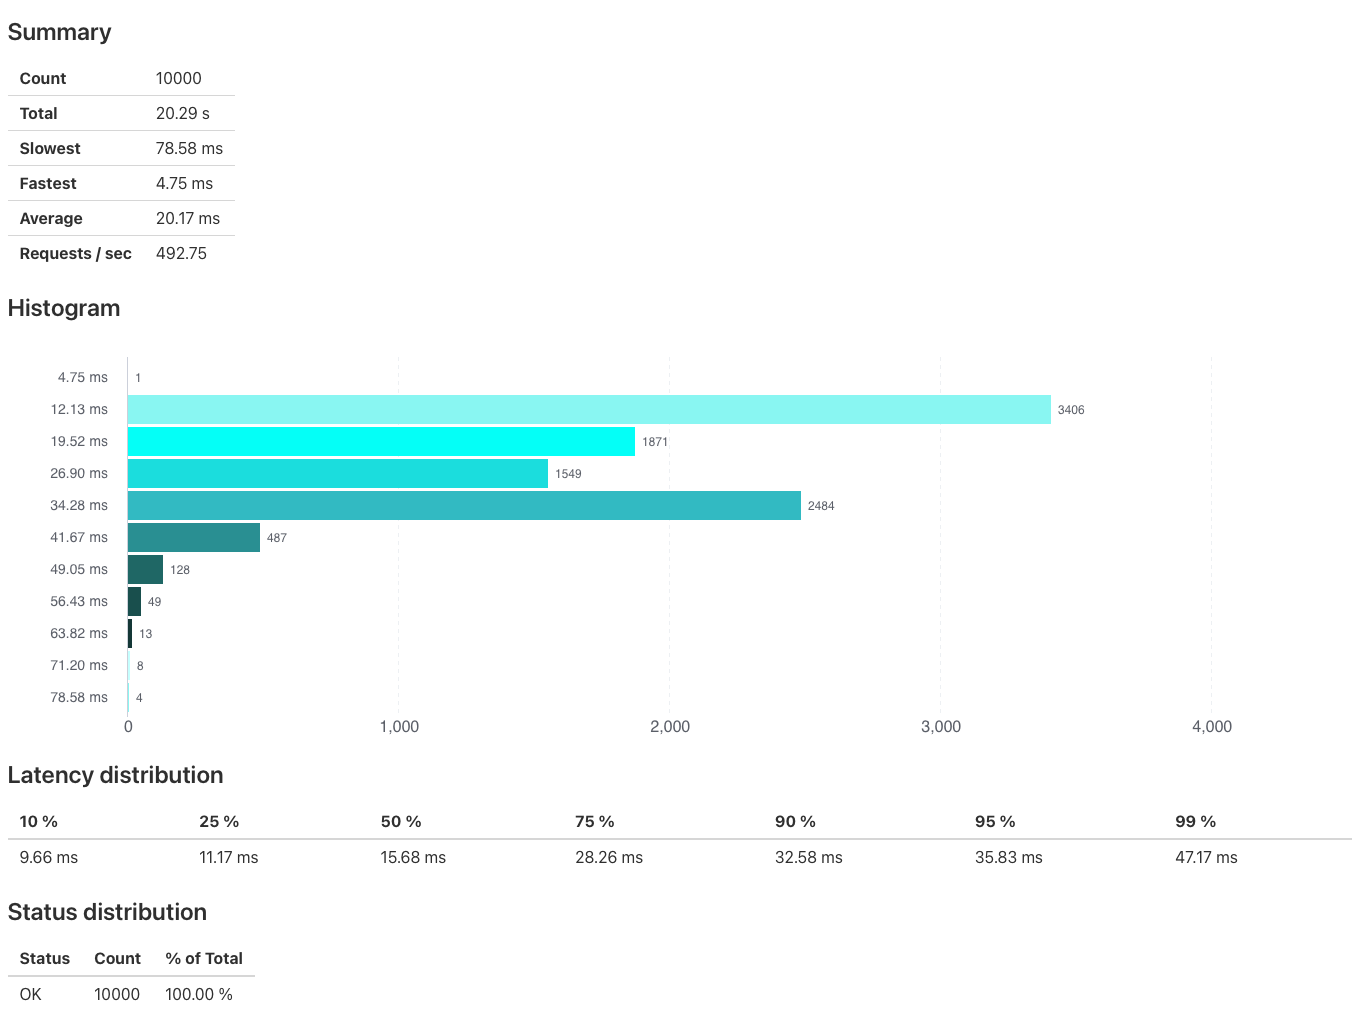
\includegraphics[scale=0.3]{images/ghz-postgres}
    \caption{Ghz mérései PostgreSQL adatbázison, gRPC}
    \label{fig:ghz-postgres}
\end{figure}

\begin{remark}
    A HTTP/2 gRPC sokkal jobban teljesített mint a HTTP/1.1 JSON.
    Ezt a diagramon is láthatjuk.
    Tehát a következtetéseink jók voltak, a HTTP/2 gRPC sokkal hatékonyabb mint a HTTP/1.1 JSON.
\end{remark}


\subsubsection{HTTP/2 gRPC, MongoDB adatbázissal \ref{fig:ghz-mongo}}
\begin{figure}[hbt!]
    \centering
    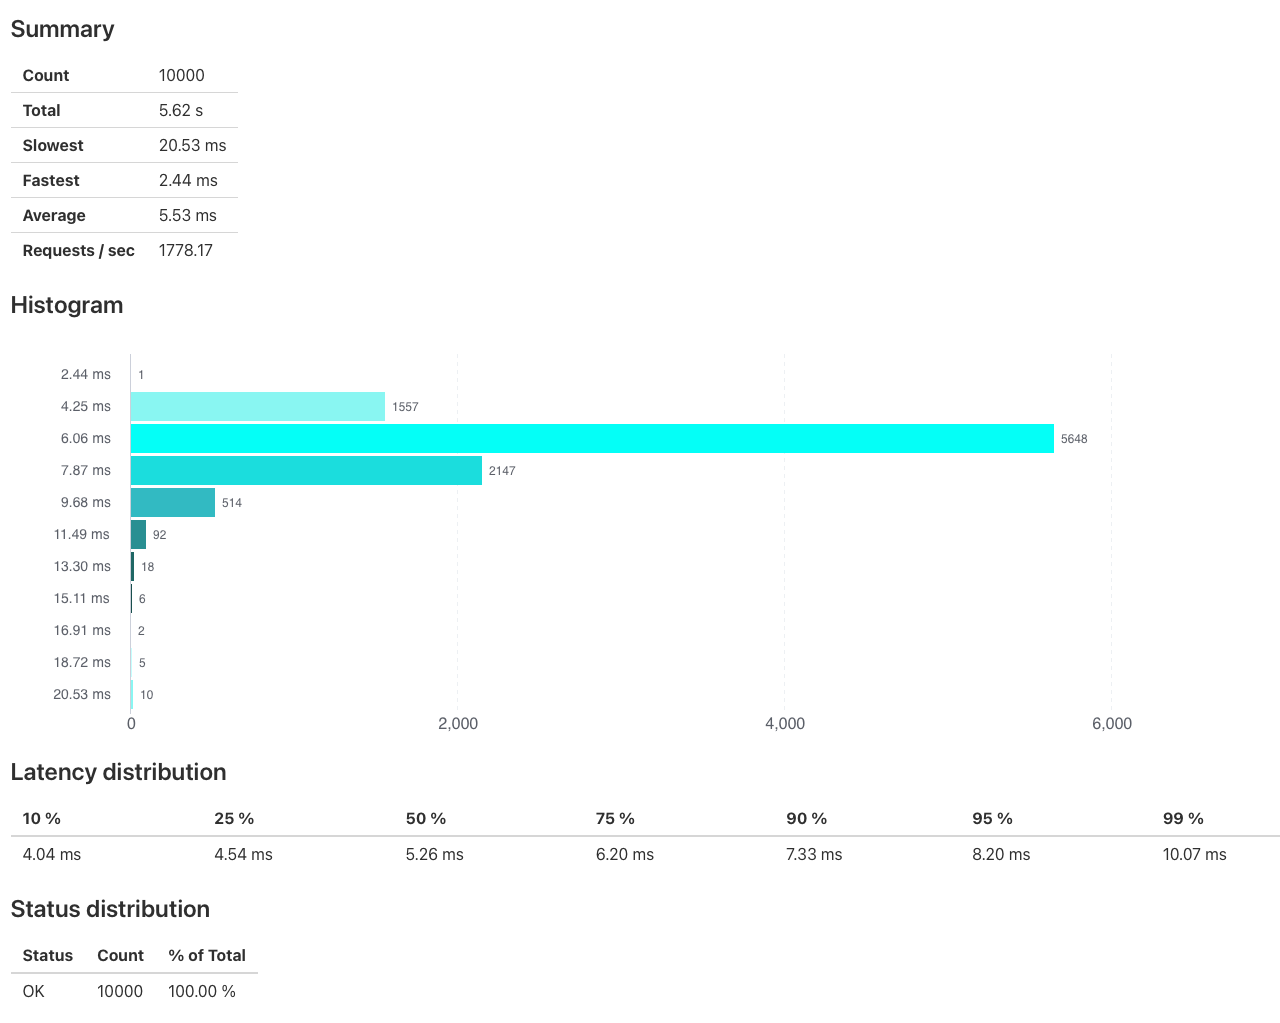
\includegraphics[scale=0.3]{images/ghz-mongo}
    \caption{Ghz mérései MongoDB adatbázison, gRPC}
    \label{fig:ghz-mongo}
\end{figure}

Összességében elmondható, hogy a gRPC a gyorsabb protokoll, és a MongoDB hatékonyabb erre a feladatra mint a PostgreSQL.



